\documentclass{beamer}

\mode<presentation>
{
  \usetheme{Warsaw}
  % or ...

  \setbeamercovered{transparent}
  % or whatever (possibly just delete it)
}

\usepackage[utf8]{inputenc}
\usepackage{amssymb}
\usepackage{amsmath}
\usepackage{subcaption}

%\DeclareMathOperator{\x}{\mathbf{x}}
\DeclareMathOperator{\e}{\mathbf{e}}
\DeclareMathOperator{\M}{\mathbf{M}}
\DeclareMathOperator{\w}{\mathbf{w}}
\newcommand{\fix}{\marginpar{FIX}}
\newcommand{\new}{\marginpar{NEW}}
\edef\polishl{\l} 



\RequirePackage{latexsym}
\RequirePackage{amsmath}
\RequirePackage{amssymb} 
\RequirePackage{color} 
\RequirePackage{bm}
\RequirePackage{color}
\RequirePackage{picinpar}

%%%%%%%% Stock standard definitions %%%%%%%%%%%%%%%

\newcommand{\wbt}{\widetilde{\mathbf{w}}}
\DeclareMathOperator{\ab}{\mathbf{a}}
\DeclareMathOperator{\abh}{\widehat{\ab}}
\DeclareMathOperator{\bb}{\mathbf{b}}
\DeclareMathOperator{\bbh}{\widehat{\bb}}
\DeclareMathOperator{\cb}{\mathbf{c}}
\DeclareMathOperator{\db}{\mathbf{d}}
\DeclareMathOperator{\eb}{\mathbf{e}}
\DeclareMathOperator{\fb}{\mathbf{f}}
\DeclareMathOperator{\gb}{\mathbf{g}}
\DeclareMathOperator{\hb}{\mathbf{h}}
\DeclareMathOperator{\ib}{\mathbf{i}}
\DeclareMathOperator{\jb}{\mathbf{j}}
\DeclareMathOperator{\kb}{\mathbf{k}}
\DeclareMathOperator{\lb}{\mathbf{l}}
\DeclareMathOperator{\mb}{\mathbf{m}}
\DeclareMathOperator{\nbb}{\mathbf{n}}
\DeclareMathOperator{\ob}{\mathbf{o}}
\DeclareMathOperator{\pb}{\mathbf{p}}
\DeclareMathOperator{\qb}{\mathbf{q}}
\DeclareMathOperator{\rb}{\mathbf{r}}
\DeclareMathOperator{\sbb}{\mathbf{s}}
\DeclareMathOperator{\tb}{\mathbf{t}}
\DeclareMathOperator{\ub}{\mathbf{u}}
\DeclareMathOperator{\vb}{\mathbf{v}}
\DeclareMathOperator{\wb}{\mathbf{w}}
\DeclareMathOperator{\xb}{\mathbf{x}}
\DeclareMathOperator{\yb}{\mathbf{y}}
\DeclareMathOperator{\zb}{\mathbf{z}}
\renewcommand{\l}{\ell}

\DeclareMathOperator{\atilde}{\tilde{\ab}}
\DeclareMathOperator{\btilde}{\tilde{\bb}}
\DeclareMathOperator{\ctilde}{\tilde{\cb}}
\DeclareMathOperator{\dtilde}{\tilde{\db}}
\DeclareMathOperator{\etilde}{\tilde{\eb}}
\DeclareMathOperator{\ftilde}{\tilde{\fb}}
\DeclareMathOperator{\gtilde}{\tilde{\gb}}
\DeclareMathOperator{\htilde}{\tilde{\hb}}
\DeclareMathOperator{\itilde}{\tilde{\ib}}
\DeclareMathOperator{\jtilde}{\tilde{\jb}}
\DeclareMathOperator{\ktilde}{\tilde{\kb}}
\DeclareMathOperator{\ltilde}{\tilde{\lb}}
\DeclareMathOperator{\mtilde}{\tilde{\mb}}
\DeclareMathOperator{\ntilde}{\tilde{\nbb}}
\DeclareMathOperator{\otilde}{\tilde{\ob}}
\DeclareMathOperator{\ptilde}{\tilde{\pb}}
\DeclareMathOperator{\qtilde}{\tilde{\qb}}
\DeclareMathOperator{\rtilde}{\tilde{\rb}}
\DeclareMathOperator{\stilde}{\tilde{\sbb}}
\DeclareMathOperator{\ttilde}{\tilde{\tb}}
\DeclareMathOperator{\utilde}{\tilde{\ub}}
\DeclareMathOperator{\vtilde}{\tilde{\vb}}
\DeclareMathOperator{\wtilde}{\tilde{\wb}}
\DeclareMathOperator{\xtilde}{\tilde{\xb}}
\DeclareMathOperator{\ytilde}{\tilde{\yb}}
\DeclareMathOperator{\ztilde}{\tilde{\zb}}

\DeclareMathOperator{\abar}{\bar{\ab}}
\DeclareMathOperator{\bbar}{\bar{\bb}}
\DeclareMathOperator{\cbar}{\bar{\cb}}
\DeclareMathOperator{\dbar}{\bar{\db}}
\DeclareMathOperator{\ebar}{\bar{\eb}}
\DeclareMathOperator{\fbar}{\bar{\fb}}
\DeclareMathOperator{\gbar}{\bar{\gb}}
\DeclareMathOperator{\hbbar}{\bar{\hb}}
\DeclareMathOperator{\ibar}{\bar{\ib}}
\DeclareMathOperator{\jbar}{\bar{\jb}}
\DeclareMathOperator{\kbar}{\bar{\kb}}
\DeclareMathOperator{\lbar}{\bar{\lb}}
\DeclareMathOperator{\mbar}{\bar{\mb}}
\DeclareMathOperator{\nbar}{\bar{\nbb}}
\DeclareMathOperator{\obar}{\bar{\ob}}
\DeclareMathOperator{\pbar}{\bar{\pb}}
\DeclareMathOperator{\qbar}{\bar{\qb}}
\DeclareMathOperator{\rbar}{\bar{\rb}}
\DeclareMathOperator{\sbar}{\bar{\sbb}}
\DeclareMathOperator{\tbar}{\bar{\tb}}
\DeclareMathOperator{\ubar}{\bar{\ub}}
\DeclareMathOperator{\vbar}{\bar{\vb}}
\DeclareMathOperator{\wbar}{\bar{\wb}}
\DeclareMathOperator{\xbar}{\bar{\xb}}
\DeclareMathOperator{\ybar}{\bar{\yb}}
\DeclareMathOperator{\zbar}{\bar{\zb}}

\DeclareMathOperator{\Ab}{\mathbf{A}}
\DeclareMathOperator{\Bb}{\mathbf{B}}
\DeclareMathOperator{\Cb}{\mathbf{C}}
\DeclareMathOperator{\Db}{\mathbf{D}}
\DeclareMathOperator{\Eb}{\mathbf{E}}
\DeclareMathOperator{\Fb}{\mathbf{F}}
\DeclareMathOperator{\Gb}{\mathbf{G}}
\DeclareMathOperator{\Hb}{\mathbf{H}}
\DeclareMathOperator{\Ib}{\mathbf{I}}
\DeclareMathOperator{\Jb}{\mathbf{J}}
\DeclareMathOperator{\Kb}{\mathbf{K}}
\DeclareMathOperator{\Lb}{\mathbf{L}}
\DeclareMathOperator{\Mb}{\mathbf{M}}
\DeclareMathOperator{\Nb}{\mathbf{N}}
\DeclareMathOperator{\Ob}{\mathbf{O}}
\DeclareMathOperator{\Pb}{\mathbf{P}}
\DeclareMathOperator{\Qb}{\mathbf{Q}}
\DeclareMathOperator{\Rb}{\mathbf{R}}
\DeclareMathOperator{\Sbb}{\mathbf{S}}
\DeclareMathOperator{\Tb}{\mathbf{T}}
\DeclareMathOperator{\Ub}{\mathbf{U}}
\DeclareMathOperator{\Vb}{\mathbf{V}}
\DeclareMathOperator{\Wb}{\mathbf{W}}
\DeclareMathOperator{\Xb}{\mathbf{X}}
\DeclareMathOperator{\Xbt}{\widetilde{\Xb}}
\DeclareMathOperator{\Xbh}{\widehat{\Xb}}
\DeclareMathOperator{\Xbs}{\widetilde{\Xb}}
\DeclareMathOperator{\Zbs}{\widetilde{\Zb}}
\DeclareMathOperator{\Kbs}{\widetilde{\Kb}}
\DeclareMathOperator{\Zbh}{\widehat{\Zb}}
\DeclareMathOperator{\Ubh}{\widehat{\Ub}}
\DeclareMathOperator{\Yb}{\mathbf{Y}}
\DeclareMathOperator{\Zb}{\mathbf{Z}}

\DeclareMathOperator{\Abar}{\bar{A}}
\DeclareMathOperator{\Bbar}{\bar{B}}
\DeclareMathOperator{\Cbar}{\bar{C}}
\DeclareMathOperator{\Dbar}{\bar{D}}
\DeclareMathOperator{\Ebar}{\bar{E}}
\DeclareMathOperator{\Fbar}{\bar{F}}
\DeclareMathOperator{\Gbar}{\bar{G}}
\DeclareMathOperator{\Hbar}{\bar{H}}
\DeclareMathOperator{\Ibar}{\bar{I}}
\DeclareMathOperator{\Jbar}{\bar{J}}
\DeclareMathOperator{\Kbar}{\bar{K}}
\DeclareMathOperator{\Lbar}{\bar{L}}
\DeclareMathOperator{\Mbar}{\bar{M}}
\DeclareMathOperator{\Nbar}{\bar{N}}
\DeclareMathOperator{\Obar}{\bar{O}}
\DeclareMathOperator{\Pbar}{\bar{P}}
\DeclareMathOperator{\Qbar}{\bar{Q}}
\DeclareMathOperator{\Rbar}{\bar{R}}
\DeclareMathOperator{\Sbar}{\bar{S}}
\DeclareMathOperator{\Tbar}{\bar{T}}
\DeclareMathOperator{\Ubar}{\bar{U}}
\DeclareMathOperator{\Vbar}{\bar{V}}
\DeclareMathOperator{\Wbar}{\bar{W}}
\DeclareMathOperator{\Xbar}{\bar{X}}
\DeclareMathOperator{\Ybar}{\bar{Y}}
\DeclareMathOperator{\Zbar}{\bar{Z}}

\DeclareMathOperator{\Abbar}{\bar{\Ab}}
\DeclareMathOperator{\Bbbar}{\bar{\Bb}}
\DeclareMathOperator{\Cbbar}{\bar{\Cb}}
\DeclareMathOperator{\Dbbar}{\bar{\Db}}
\DeclareMathOperator{\Ebbar}{\bar{\Eb}}
\DeclareMathOperator{\Fbbar}{\bar{\Fb}}
\DeclareMathOperator{\Gbbar}{\bar{\Gb}}
\DeclareMathOperator{\Hbbar}{\bar{\Hb}}
\DeclareMathOperator{\Ibbar}{\bar{\Ib}}
\DeclareMathOperator{\Jbbar}{\bar{\Jb}}
\DeclareMathOperator{\Kbbar}{\bar{\Kb}}
\DeclareMathOperator{\Lbbar}{\bar{\Lb}}
\DeclareMathOperator{\Mbbar}{\bar{\Mb}}
\DeclareMathOperator{\Nbbar}{\bar{\Nb}}
\DeclareMathOperator{\Obbar}{\bar{\Ob}}
\DeclareMathOperator{\Pbbar}{\bar{\Pb}}
\DeclareMathOperator{\Qbbar}{\bar{\Qb}}
\DeclareMathOperator{\Rbbar}{\bar{\Rb}}
\DeclareMathOperator{\Sbbar}{\bar{\Sb}}
\DeclareMathOperator{\Tbbar}{\bar{\Tb}}
\DeclareMathOperator{\Ubbar}{\bar{\Ub}}
\DeclareMathOperator{\Vbbar}{\bar{\Vb}}
\DeclareMathOperator{\Wbbar}{\bar{\Wb}}
\DeclareMathOperator{\Xbbar}{\bar{\Xb}}
\DeclareMathOperator{\Ybbar}{\bar{\Yb}}
\DeclareMathOperator{\Zbbar}{\bar{\Zb}}

\DeclareMathOperator{\Ahat}{\widehat{A}}
\DeclareMathOperator{\Bhat}{\widehat{B}}
\DeclareMathOperator{\Chat}{\widehat{C}}
\DeclareMathOperator{\Dhat}{\widehat{D}}
\DeclareMathOperator{\Ehat}{\widehat{E}}
\DeclareMathOperator{\Fhat}{\widehat{F}}
\DeclareMathOperator{\Ghat}{\widehat{G}}
\DeclareMathOperator{\Hhat}{\widehat{H}}
\DeclareMathOperator{\Ihat}{\widehat{I}}
\DeclareMathOperator{\Jhat}{\widehat{J}}
\DeclareMathOperator{\Khat}{\widehat{K}}
\DeclareMathOperator{\Lhat}{\widehat{L}}
\DeclareMathOperator{\Mhat}{\widehat{M}}
\DeclareMathOperator{\Nhat}{\widehat{N}}
\DeclareMathOperator{\Ohat}{\widehat{O}}
\DeclareMathOperator{\Phat}{\widehat{P}}
\DeclareMathOperator{\Qhat}{\widehat{Q}}
\DeclareMathOperator{\Rhat}{\widehat{R}}
\DeclareMathOperator{\Shat}{\widehat{S}}
\DeclareMathOperator{\That}{\widehat{T}}
\DeclareMathOperator{\Uhat}{\widehat{U}}
\DeclareMathOperator{\Vhat}{\widehat{V}}
\DeclareMathOperator{\What}{\widehat{W}}
\DeclareMathOperator{\Xhat}{\widehat{X}}
\DeclareMathOperator{\Yhat}{\widehat{Y}}
\DeclareMathOperator{\Zhat}{\widehat{Z}}

\DeclareMathOperator{\Abhat}{\widehat{\Ab}}
\DeclareMathOperator{\Bbhat}{\widehat{\Bb}}
\DeclareMathOperator{\Cbhat}{\widehat{\Cb}}
\DeclareMathOperator{\Dbhat}{\widehat{\Db}}
\DeclareMathOperator{\Ebhat}{\widehat{\Eb}}
\DeclareMathOperator{\Fbhat}{\widehat{\Fb}}
\DeclareMathOperator{\Gbhat}{\widehat{\Gb}}
\DeclareMathOperator{\Hbhat}{\widehat{\Hb}}
\DeclareMathOperator{\Ibhat}{\widehat{\Ib}}
\DeclareMathOperator{\Jbhat}{\widehat{\Jb}}
\DeclareMathOperator{\Kbhat}{\widehat{\Kb}}
\DeclareMathOperator{\Lbhat}{\widehat{\Lb}}
\DeclareMathOperator{\Mbhat}{\widehat{\Mb}}
\DeclareMathOperator{\Nbhat}{\widehat{\Nb}}
\DeclareMathOperator{\Obhat}{\widehat{\Ob}}
\DeclareMathOperator{\Pbhat}{\widehat{\Pb}}
\DeclareMathOperator{\Qbhat}{\widehat{\Qb}}
\DeclareMathOperator{\Rbhat}{\widehat{\Rb}}
\DeclareMathOperator{\Sbhat}{\widehat{\Sb}}
\DeclareMathOperator{\Tbhat}{\widehat{\Tb}}
\DeclareMathOperator{\Ubhat}{\widehat{\Ub}}
\DeclareMathOperator{\Vbhat}{\widehat{\Vb}}
\DeclareMathOperator{\Wbhat}{\widehat{\Wb}}
\DeclareMathOperator{\Xbhat}{\widehat{\Xb}}
\DeclareMathOperator{\Ybhat}{\widehat{\Yb}}
\DeclareMathOperator{\Zbhat}{\widehat{\Zb}}

\DeclareMathOperator{\Acal}{\mathcal{A}}
\DeclareMathOperator{\Bcal}{\mathcal{B}}
\DeclareMathOperator{\Ccal}{\mathcal{C}}
\DeclareMathOperator{\Dcal}{\mathcal{D}}
\DeclareMathOperator{\Ecal}{\mathcal{E}}
\DeclareMathOperator{\Fcal}{\mathcal{F}}
\DeclareMathOperator{\Gcal}{\mathcal{G}}
\DeclareMathOperator{\Hcal}{\mathcal{H}}
\DeclareMathOperator{\Ical}{\mathcal{I}}
\DeclareMathOperator{\Jcal}{\mathcal{J}}
\DeclareMathOperator{\Kcal}{\mathcal{K}}
\DeclareMathOperator{\Lcal}{\mathcal{L}}
\DeclareMathOperator{\Mcal}{\mathcal{M}}
\DeclareMathOperator{\Ncal}{\mathcal{N}}
\DeclareMathOperator{\Ocal}{\mathcal{O}}
\DeclareMathOperator{\Pcal}{\mathcal{P}}
\DeclareMathOperator{\Qcal}{\mathcal{Q}}
\DeclareMathOperator{\Rcal}{\mathcal{R}}
\DeclareMathOperator{\Scal}{\mathcal{S}}
\DeclareMathOperator{\Scalt}{\widetilde{\Scal}}
\DeclareMathOperator{\Tcal}{\mathcal{T}}
\DeclareMathOperator{\Ucal}{\mathcal{U}}
\DeclareMathOperator{\Vcal}{\mathcal{V}}
\DeclareMathOperator{\Wcal}{\mathcal{W}}
\DeclareMathOperator{\Xcal}{\mathcal{X}}
\DeclareMathOperator{\Ycal}{\mathcal{Y}}
\DeclareMathOperator{\Zcal}{\mathcal{Z}}

\DeclareMathOperator{\Atilde}{\widetilde{A}}
\DeclareMathOperator{\Btilde}{\widetilde{B}}
\DeclareMathOperator{\Ctilde}{\widetilde{C}}
\DeclareMathOperator{\Dtilde}{\widetilde{D}}
\DeclareMathOperator{\Etilde}{\widetilde{E}}
\DeclareMathOperator{\Ftilde}{\widetilde{F}}
\DeclareMathOperator{\Gtilde}{\widetilde{G}}
\DeclareMathOperator{\Htilde}{\widetilde{H}}
\DeclareMathOperator{\Itilde}{\widetilde{I}}
\DeclareMathOperator{\Jtilde}{\widetilde{J}}
\DeclareMathOperator{\Ktilde}{\widetilde{K}}
\DeclareMathOperator{\Ltilde}{\widetilde{L}}
\DeclareMathOperator{\Mtilde}{\widetilde{M}}
\DeclareMathOperator{\Ntilde}{\widetilde{N}}
\DeclareMathOperator{\Otilde}{\widetilde{O}}
\DeclareMathOperator{\Ptilde}{\widetilde{P}}
\DeclareMathOperator{\Qtilde}{\widetilde{Q}}
\DeclareMathOperator{\Rtilde}{\widetilde{R}}
\DeclareMathOperator{\Stilde}{\widetilde{S}}
\DeclareMathOperator{\Ttilde}{\widetilde{T}}
\DeclareMathOperator{\Utilde}{\widetilde{U}}
\DeclareMathOperator{\Vtilde}{\widetilde{V}}
\DeclareMathOperator{\Wtilde}{\widetilde{W}}
\DeclareMathOperator{\Xtilde}{\widetilde{X}}
\DeclareMathOperator{\Ytilde}{\widetilde{Y}}
\DeclareMathOperator{\Ztilde}{\widetilde{Z}}


%%%%%%%% Widely accepted definitions %%%%%%%%%%%%%%%

\DeclareMathOperator{\CC}{\mathbb{C}} % Complex numbers
\DeclareMathOperator{\EE}{\mathbb{E}} % Expectation
\DeclareMathOperator{\KK}{\mathbb{K}} % Arbitrary field
\DeclareMathOperator{\MM}{\mathbb{M}} % Median
\DeclareMathOperator{\NN}{\mathbb{N}} % Natural numbers
\DeclareMathOperator{\PP}{\mathbb{P}} % Probability
\DeclareMathOperator{\QQ}{\mathbb{Q}} % Rationals
\DeclareMathOperator{\RR}{\mathbb{R}} % Real numbers 
\DeclareMathOperator{\ZZ}{\mathbb{Z}} % Integers

\DeclareMathOperator{\one}{\mathbf{1}}  % Identity
\DeclareMathOperator{\zero}{\mathbf{0}} % Zero
\DeclareMathOperator{\TRUE}{\mathbf{TRUE}}  % True
\DeclareMathOperator{\FALSE}{\mathbf{FALSE}}  % False

\DeclareMathOperator*{\mini}{\mathop{\mathrm{minimize}}}
\DeclareMathOperator*{\maxi}{\mathop{\mathrm{maximize}}}
\DeclareMathOperator*{\argmin}{\mathop{\mathrm{argmin}}}
\DeclareMathOperator*{\argmax}{\mathop{\mathrm{argmax}}}
\DeclareMathOperator*{\argsup}{\mathop{\mathrm{argsup}}}
\DeclareMathOperator*{\arginf}{\mathop{\mathrm{arginf}}}
\DeclareMathOperator{\sgn}{\mathop{\mathrm{sign}}}
\DeclareMathOperator{\sign}{\mathop{\mathrm{sign}}}
\DeclareMathOperator{\tr}{\mathop{\mathrm{tr}}}
\DeclareMathOperator{\rank}{\mathop{\mathrm{rank}}}
\DeclareMathOperator{\traj}{\mathop{\mathrm{Traj}}}

%%%%%%%% Bold Greek Letters %%%%%%%%%%%%%%%
\DeclareMathOperator{\sigmab}{\bm{\sigma}}
\DeclareMathOperator{\Sigmab}{\mathbf{\Sigma}}


%%%%%%%% Mess around with LaTeX %%%%%%%%%%%%%%%

%% Some style files might actually define these variables.
%% So don't mess with them if they are already defined

\ifx\BlackBox\undefined
\newcommand{\BlackBox}{\rule{1.5ex}{1.5ex}}  % end of proof
\fi

\ifx\proof\undefined
\newenvironment{proof}{\par\noindent{\bf Proof\ }}{\hfill\BlackBox\\[2mm]}
% \else
% \renewenvironment{proof}{\par\noindent{\bf Proof\ }}{\hfill\BlackBox\\[2mm]}
\fi

%Trying to put all on Section track
%\makeatletter
%\@addtoreset{equation}{section}
%\def\theequation{\thesection.\arabic{equation}}
%\def\thetheorem{\thesection.\arabic{theorem}}
%\makeatother

%the below clashes with the previous defs of them... 
%in the style files
%\newtheorem{theorem}{Theorem}[section]
%\newtheorem{lemma}[theorem]{Lemma}
%\newtheorem{corollary}[theorem]{Corollary}
%\newtheorem{conjecture}[conjecture]{Conjecture}


%%%%%%%% Utility functions %%%%%%%%%%%%%%%

\newcommand{\eq}[1]{(\ref{#1})} 
\newcommand{\mymatrix}[2]{\left[\begin{array}{#1} #2 \end{array}\right]}
\newcommand{\mychoose}[2]{\left(\begin{array}{c} #1 \\ #2 \end{array}\right)}
\newcommand{\mydet}[1]{\det\left[ #1 \right]}
\newcommand{\sembrack}[1]{[\![#1]\!]}

\newcommand{\ea}{\emph{et al. }}
\newcommand{\eg}{\emph{e.g. }}
\newcommand{\ie}{\emph{i.e., }}

\newcommand{\mnote}[1]{\marginpar{#1}}
\newcommand{\note}[1]{{\bf {#1}}}

%%%%%%%% Specific symbols for this project %%%%%%%%%%%%%%%

\DeclareMathOperator{\half}{\frac{1}{2}}

\newcommand{\Ref}[1]{\hfill\Green{[#1]}}
\DeclareMathOperator{\XX}{\mathcal{X}}
\newcommand{\ar}{\implies}
\newcommand{\yh}{\hat{y}}
\DeclareMathOperator{\lan}{\langle}
\DeclareMathOperator{\ran}{\rangle}

\DeclareMathOperator{\dc}{\mathrm{dc}}

\DeclareMathOperator{\Utb}{\widetilde{\Ub}}
\DeclareMathOperator{\Stb}{\widetilde{\Sbb}}

\ifx\Brown\undefined
\definecolor{brown}{rgb}{0.5,0.1,0.1}
\newcommand{\Brown}[1]{\color{brown}{#1}\color{black}}
\fi

\ifx\Red\undefined
\definecolor{red}{rgb}{1.0,0,0}
\newcommand{\Red}[1]{\color{red}{#1}\color{black}}
\fi

\ifx\Green\undefined
\definecolor{green}{rgb}{0,0.4,0}
\newcommand{\Green}[1]{\color{green}{#1}\color{black}}
\fi

\ifx\Blue\undefined
\definecolor{blue}{rgb}{0,0,1.0}
\newcommand{\Blue}[1]{\color{blue}{#1}\color{black}}
\fi



\newcommand{\beq}{\begin{equation}}
\newcommand{\eeq}{\end{equation}}
\newcommand{\beh}{\begin{conjecture}}
\newcommand{\eeh}{\end{conjecture}}
\newcommand\bel{\begin{lemma}}
\newcommand\eel{\end{lemma}}
\newcommand\bet{\begin{theoreme}}
\newcommand\eet{\end{theoreme}}
\newcommand\bex{\begin{example}}
\newcommand\eex{\end{example}}
\newcommand\bed{\begin{definition}}
\newcommand\eed{\end{definition}}
\newcommand\bep{\begin{proposition}}
\newcommand\eep{\end{proposition}}
\newcommand\ber{\begin{remark}}
\newcommand\eer{\end{remark}}
\newcommand\bec{\begin{corollary}}
\newcommand\eec{\end{corollary}}
%\newcommand\proof{\noindent {\bf Proof.}\ \ }
\newcommand\qed{\hfill$\Box$\medskip}
\newcommand\cP{{\mathcal P}}
\newcommand\cJ{{\mathcal J}}
\newcommand\cD{{\mathcal D}}
\newcommand\cC{{\mathcal C}}
\newcommand\cO{{\mathcal O}}
\newcommand\cS{{\mathcal S}}
\newcommand\cT{{\mathcal T}}
\newcommand\cV{{\mathcal V}}
\newcommand\cW{{\mathcal W}}
\newcommand\cY{{\mathcal Y}}
\newcommand\cF{{\mathcal F}}
\newcommand\cU{{\mathcal U}}
\newcommand\cE{{\mathcal E}}
\newcommand\cG{{\mathcal G}}
\newcommand\cB{{\mathcal B}}
\newcommand\cI{{\rm I}}
\newcommand\cN{{\mathcal N}}
\newcommand\cM{{\mathcal M}}
\newcommand\cA{{\mathcal A}}
\newcommand\cQ{{\mathcal Q}}
\newcommand\cK{{\mathcal K}}
\newcommand\cZ{{\mathcal Z}}
\newcommand\CAP{{\rm cap}}
\newcommand\ENT{{\rm ent}}
\newcommand\gr{{\rm gr}}

\def\qq{{\mathbb Q}}
\def\ff{{\mathbb F}}
\def\rr{{\mathbb R}}
\def\zz{{\mathbb Z}}
\def\cc{{\mathbb C}}
\def\nn{{\mathbb N}}
\def\kk{{\mathbb K}}
\def\ee{{\mathbb E}}
\def\ww{{\mathbb W}}
\def\hh{{\mathbb H}}
\def\ss{{\mathbb S}}
\def\tt{{\mathbb T}}
\def\pp{{\mathbb P}}



% \newtheorem{theoreme}{Theorem} %[section]
% \newtheorem{proposition}[theoreme]{Proposition}
% \newtheorem{lemma}[theoreme]{Lemma}
% \newtheorem{definition}[theoreme]{Definition}
% \newtheorem{corollary}[theoreme]{Corollary}
% \newtheorem{remark}[theoreme]{Remark}
% \newtheorem{example}[theoreme]{Example}
% \newtheorem{examples}[theoreme]{Examples}
% \newtheorem{conjecture}[theoreme]{Conjecture}
% \newtheorem{conjecture}{Conjecture}
\newcommand{\beq}{\begin{equation}}
\newcommand{\eeq}{\end{equation}}
\newcommand{\beh}{\begin{Conjecture}}
\newcommand{\eeh}{\end{Conjecture}}
\newcommand\bel{\begin{Lemma}}
\newcommand\eel{\end{Lemma}}
\newcommand\bet{\begin{Theorem}}
\newcommand\eet{\end{Theorem}}
\newcommand\bex{\begin{Example}}
\newcommand\eex{\end{Example}}
\newcommand\bed{\begin{Definition}}
\newcommand\eed{\end{Definition}}
\newcommand\bep{\begin{Proposition}}
\newcommand\eep{\end{Proposition}}
\newcommand\ber{\begin{Remark}}
\newcommand\eer{\end{Remark}}
\newcommand\bec{\begin{Corollary}}
\newcommand\eec{\end{Corollary}}
%\newcommand\proof{\noindent {\bf Proof.}\ \ }
%\newcommand\qed{\hfill$\Box$\medskip}
\newcommand\cP{{\mathcal P}}
\newcommand\cJ{{\mathcal J}}
\newcommand\cD{{\mathcal D}}
\newcommand\cC{{\mathcal C}}
\newcommand\cO{{\mathcal O}}
\newcommand\cS{{\mathcal S}}
\newcommand\cT{{\mathcal T}}
\newcommand\cV{{\mathcal V}}
\newcommand\cW{{\mathcal W}}
\newcommand\cY{{\mathcal Y}}
\newcommand\cF{{\mathcal F}}
\newcommand\cU{{\mathcal U}}
\newcommand\cE{{\mathcal E}}
\newcommand\cG{{\mathcal G}}
\newcommand\cB{{\mathcal B}}
\newcommand\cI{{\rm I}}
\newcommand\cN{{\mathcal N}}
\newcommand\cM{{\mathcal M}}
\newcommand\cA{{\mathcal A}}
\newcommand\cQ{{\mathcal Q}}
\newcommand\cK{{\mathcal K}}
\newcommand\cZ{{\mathcal Z}}
\newcommand\CAP{{\rm cap}}
\newcommand\ENT{{\rm ent}}
\newcommand\gr{{\rm gr}}

\def\qq{{\mathbb Q}}
\def\ff{{\mathbb F}}
\def\rr{{\mathbb R}}
\def\zz{{\mathbb Z}}
\def\cc{{\mathbb C}}
\def\nn{{\mathbb N}}
\def\kk{{\mathbb K}}
\def\ee{{\mathbb E}}
\def\ww{{\mathbb W}}
\def\hh{{\mathbb H}}
\def\ss{{\mathbb S}}
\def\tt{{\mathbb T}}
\def\pp{{\mathbb P}}


\setkeys{Gin}{width=0.7\textwidth}

\title[Quantifying Text Interestingness]{An Information Theoretic
    Approach to Quantifying Text Interestingness}  


\author{Michał Dereziński, Khashayar Rohanimanesh}

\begin{document}

\begin{frame}
  \titlepage
\end{frame}

\linespread{1.3}

\section{Introduction}
\subsection{Problem Statement}
\begin{frame}
\frametitle{Finding Interesting Products on eBay}
\begin{itemize}
\item {\bf Goal:} Increase user engagement when shopping online.
\item {\bf Solution:} Display ads for products that are {\em unique},
  {\em surprising}, {\em interesting}. 
\item Users are unlikely to buy such products, but may still browse
  them and click on the ads. 
\end{itemize}
\end{frame}

\begin{frame}
\frametitle{Example: Random iPhone Cases}
\begin{figure}
\centering
\makebox[\textwidth][c]{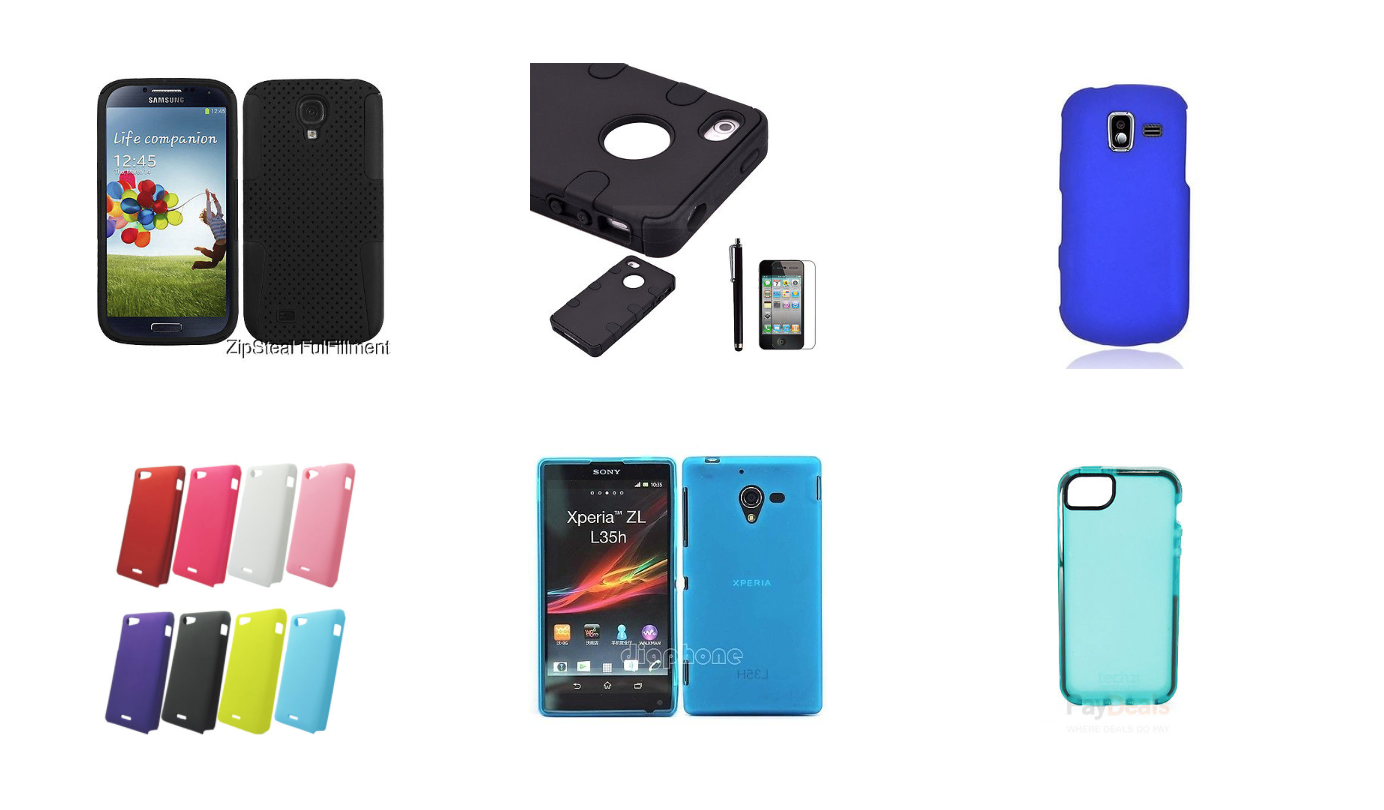
\includegraphics[width=\textwidth]{figures/boring.png}}
\label{fig:boring}
\end{figure}
\end{frame}

\begin{frame}
\frametitle{Example: Interesting iPhone Cases}
\begin{figure}
\centering
\makebox[\textwidth][c]{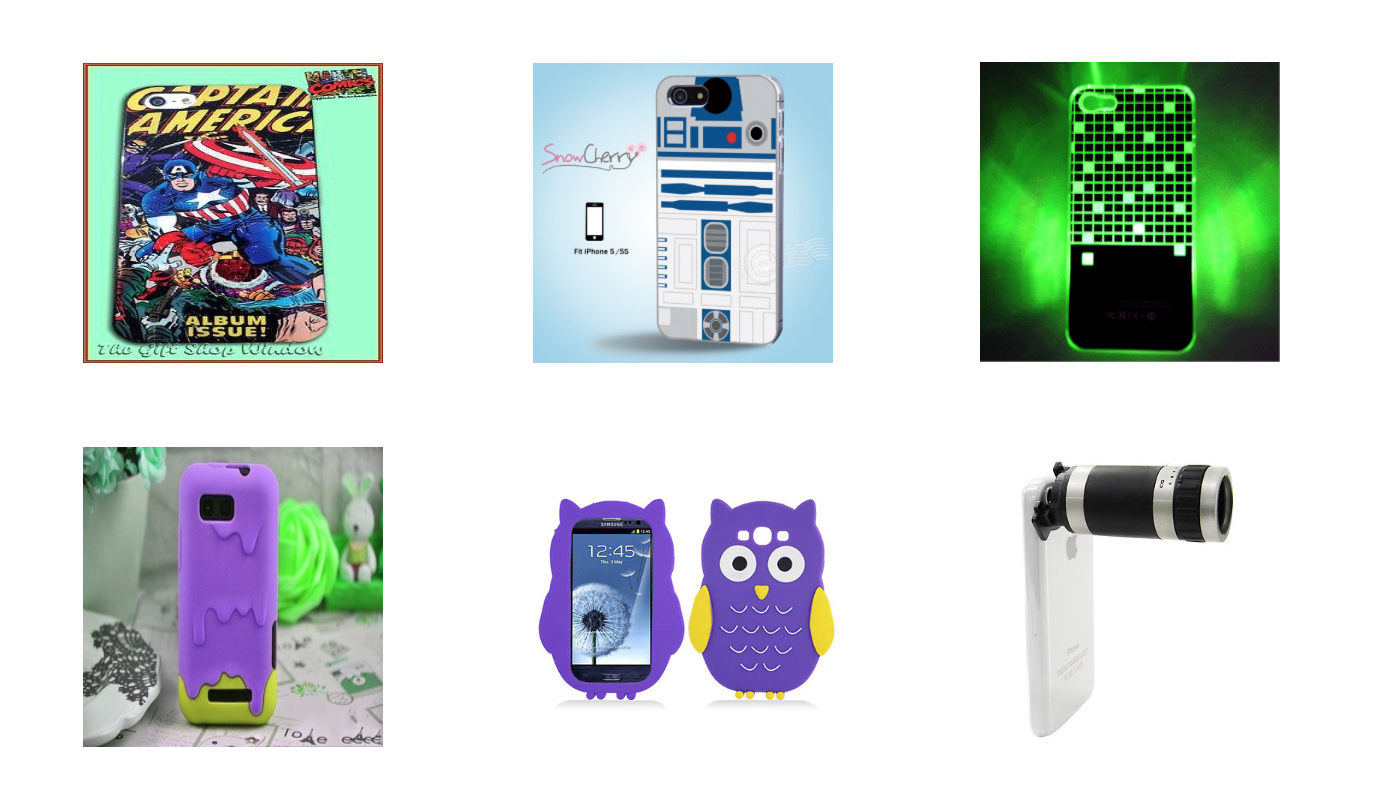
\includegraphics[width=\textwidth]{figures/interesting.png}}
\label{fig:interesting}
\end{figure}
\end{frame}

\subsection{Hypothesis}

\begin{frame}
\frametitle{Interestingness as Text Diversity}
\begin{itemize}
\item We used eBay listing titles as the features.
\item Our hypothesis is that often an interesting concept is generated
  by mixing a diverse set of topics.
\item We can identify those topics from the words appearing in the
  product title (usually 10-12 words).
\end{itemize}
\end{frame}

\begin{frame}
\frametitle{Example: Diversity in Product Titles}
\begin{figure}
\label{fig:ebay-products}
        \centering
         \begin{subfigure}[b]{0.3\textwidth}
        	        \centering
                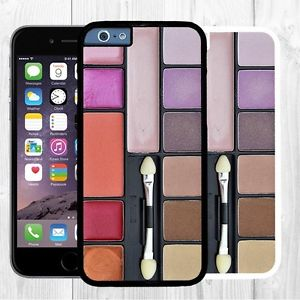
\includegraphics[width=25mm]{figures/eyeshadow-iphone-case.jpg}
                \caption{\textcolor{red}{{\bf Eyeshadow}} Palettes for \textcolor{red}{{\bf iPhone}} 6 case}
                \label{fig:eyeshadow-iphone-case}
        \end{subfigure}
              ~ %add desired spacing between images, e. g. ~, \quad, \qquad, \hfill etc.
          %(or a blank line to force the subfigure onto a new line)
        \begin{subfigure}[b]{0.3\textwidth}
		 \centering
                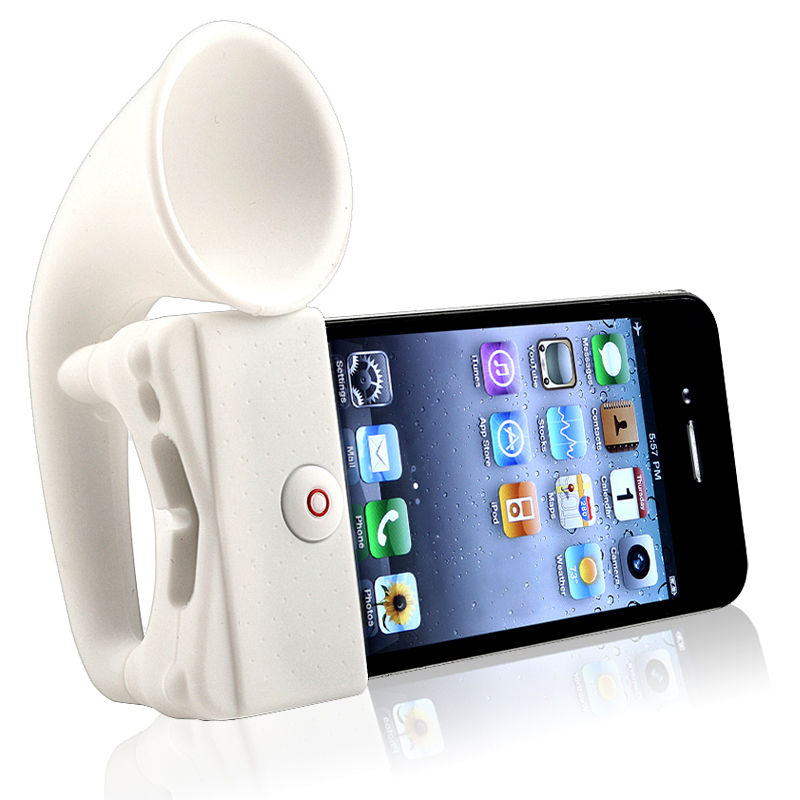
\includegraphics[width=25mm]{figures/horn-iphone-speaker.jpg}
\caption{White Silicone \textcolor{red}{{\bf Horn}} Stand Speaker for Apple \textcolor{red}{{\bf iPhone}} 4/ 4S}                \label{fig:zeppelin-speaker}
        \end{subfigure}
       ~ %add desired spacing between images, e. g. ~, \quad, \qquad, \hfill etc.
          %(or a blank line to force the subfigure onto a new line)
        \begin{subfigure}[b]{0.3\textwidth}
		 \centering
                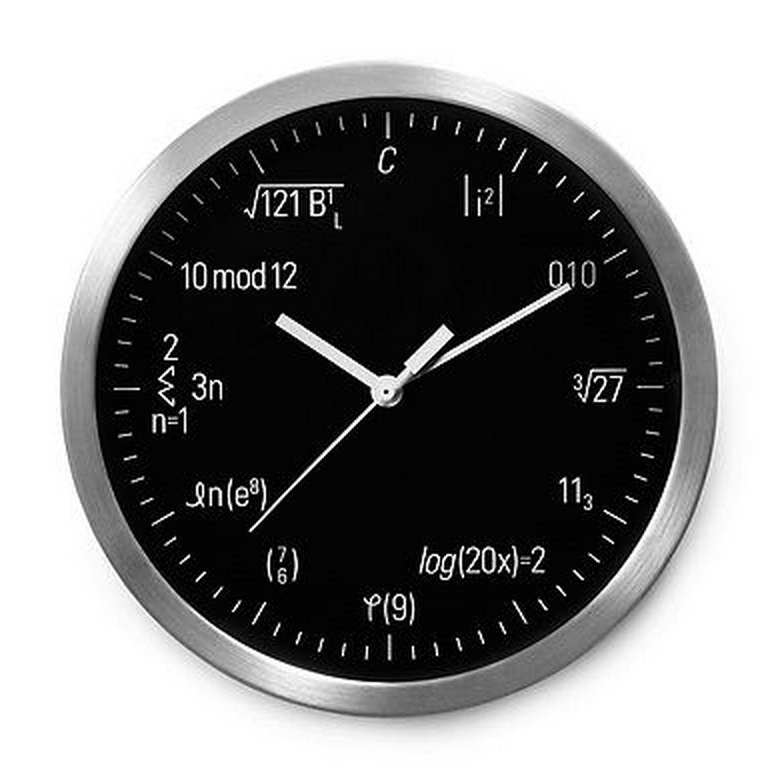
\includegraphics[width=30mm]{figures/geeky-clock.jpg}
\caption{\textcolor{red}{{\bf Equation}} Wall \textcolor{red}{{\bf
      Clock}} Gifts for Math Gurus}                
\label{fig:geeky-clock}
        \end{subfigure}
       % \caption{A collection of unique/interesting {\em eBay}
       % products. Highlighted keywords demonstrate how the text
       % associated with such products could span multiple diverse
       % topics.}
\end{figure}
\end{frame}

\subsection{Model Assumptions}

\begin{frame}
\frametitle{Distributional Word Representation}
\begin{itemize}
\item Each word in the vocabulary $V$ is mapped to a probability
  distribution over a fixed domain $T$.
\item Often, we start by a {\bf co-occurrence matrix} $\cM_{|V|\times|T|}$
  where each row represents a co-occurrence of a word with the set
  $T$. 
\item For $T=V$, we obtain the familiar {\em word-to-word}
  co-occurrence representation.
\item We chose to use {\bf topic modeling} where $T$ is the set of
  topics learned over a document corpus by {\em Latent Dirichlet
    Allocation}. 
\end{itemize}
\end{frame}

\begin{frame}
\frametitle{The Observer's Model}
\begin{itemize}
\item Consider an Observer reading a text $W=\{w_1,...,w_k\}$. 
\item The Observer represents the meaning of each word $w_i$ with a probability
  distribution $P_{i}$ over a set of topics $T$.
\item The Observer's {\em knowledge} is matrix $\cM_{|V|\times|T|}$ coming
  from an LDA topic model trained on a separate corpus of documents.
\item We will address two questions:
\begin{enumerate}
\item How should the Observer choose $P_{i}$ given $W$, knowing
  $\cM_{|V|\times|T|}$?
\item Given $\cP_{W}=\{P_{1},...,P_{k}\}$, knowing
  $\cM_{|V|\times|T|}$, how should the Observer measure diversity of $W$?
\end{enumerate}
\end{itemize}
\end{frame}

\section{The Observer's Model}

\subsection{Information Diversity}

\begin{frame}
\frametitle{Jensen-Shannon Divergence}
\bed
The classical Jensen-Shannon Divergence between distributions $P$ and
$Q$ is defined (denoting $M=\frac{1}{2}(P+Q)$) as
\[D_{JS}(P,Q) = \frac{1}{2}\left(D_{KL}(P\|M)+D_{KL}(Q\|M)\right).\]
\eed
\bed
Generalized Jensen-Shannon Divergence for  $\cP=\{P_{1},...,P_{k}\}$
and weights $d_1+...+d_k=1$ is defined (denoting $M=\sum_{i=1}^k d_i
P_i$) as
\[D_{JS}(\Sigma d_iP_i) = \sum_{i=1}^k d_i D_{KL}(P_i\|M).\] 
\eed
\end{frame}

\begin{frame}
\frametitle{Information Diversity}
\bed\label{importance}
Given a distribution $P_i$, its {\sl importance} with respect to a
prior distribution $P$ is defined as $D_i = D_{KL}(P_i\|P)$.
\eed
\begin{itemize}
\item Here, $P_i$ represents a topic distribution for some word
  $w_i$. 
\item We can write it as a conditional distribution
  $\pp(t|w_i,\cB)$, where $\cB$ represents background knowledge. 
\item In this context, the prior $P$ would correspond to
  $\pp(t|\cB)$. 
\item {\em Importance} represents the amount of information obtained
  by conditioning on $w_i$.
\end{itemize}
\end{frame}

\begin{frame}
\frametitle{Information Diversity, cont.}
\bed\label{diversity}
We define the Jensen-Shannon Information Diversity of $\cP$ with
respect to prior $P$ as $\mbox{JSID}_P(\cP)=D_{JS}(\Sigma d_i P_i)$
where $d_{i}=\frac{D_{i}}{\sum D_{j}}$ are the normalized importances.
\eed
\bet\label{entropy}
Let $\cP$ be such that each $P_i$ has a singleton support. Assume that
the prior $U$ is in this case uniform. Then, 
$JSID_U(\cP)=H(P_S)$,
where $P_S$ corresponds to the overall distribution in the set
$S$, and $H$ denotes Shannon entropy.
\eet
\end{frame}

\begin{frame}
\frametitle{Information Diversity: Example}
\begin{figure}
\label{fig:diversity}
        \centering
         \begin{subfigure}[b]{0.45\textwidth}
        	        \centering
                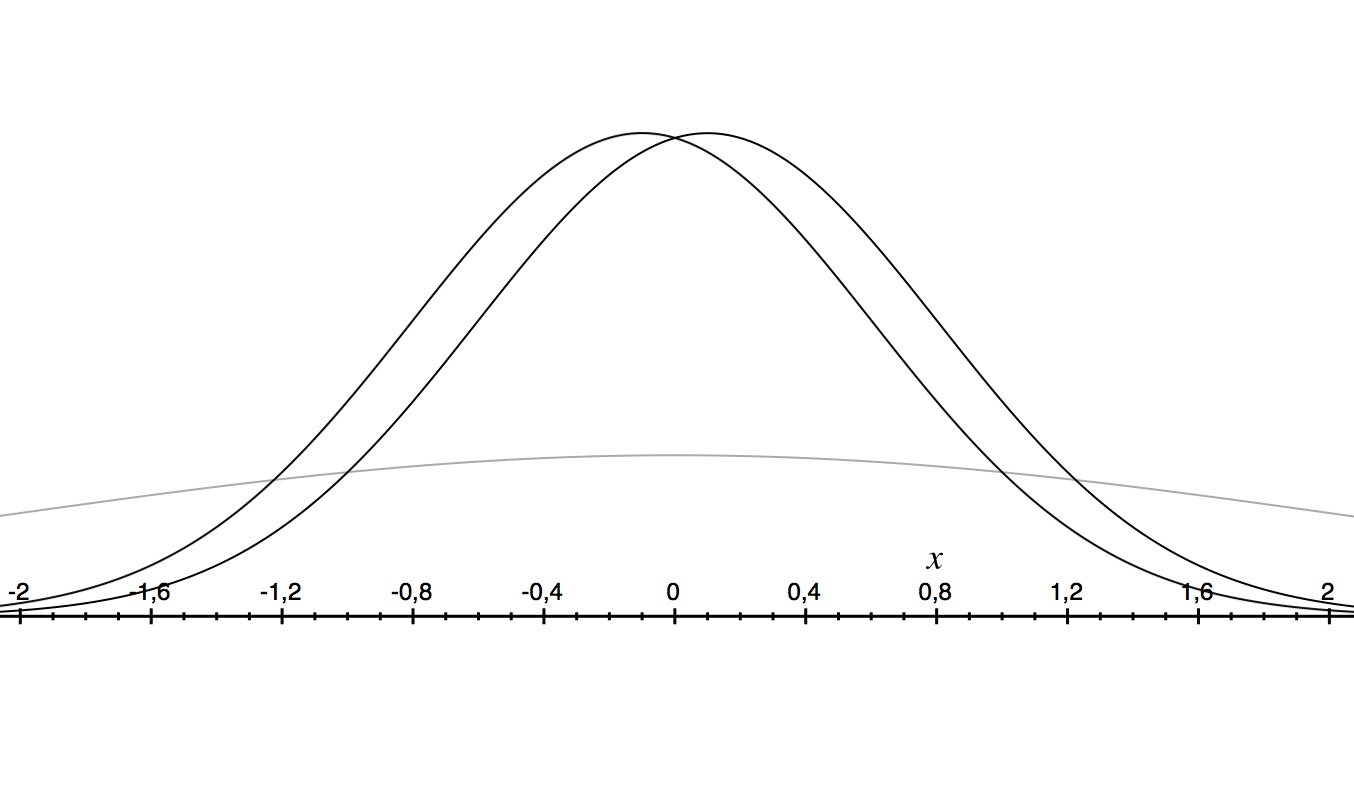
\includegraphics[width=50mm]{figures/diversity1.jpg}
                \caption{Low diversity}
        \end{subfigure}
              ~ %add desired spacing between images, e. g. ~, \quad, \qquad, \hfill etc.
          %(or a blank line to force the subfigure onto a new line)
        \begin{subfigure}[b]{0.45\textwidth}
		 \centering
                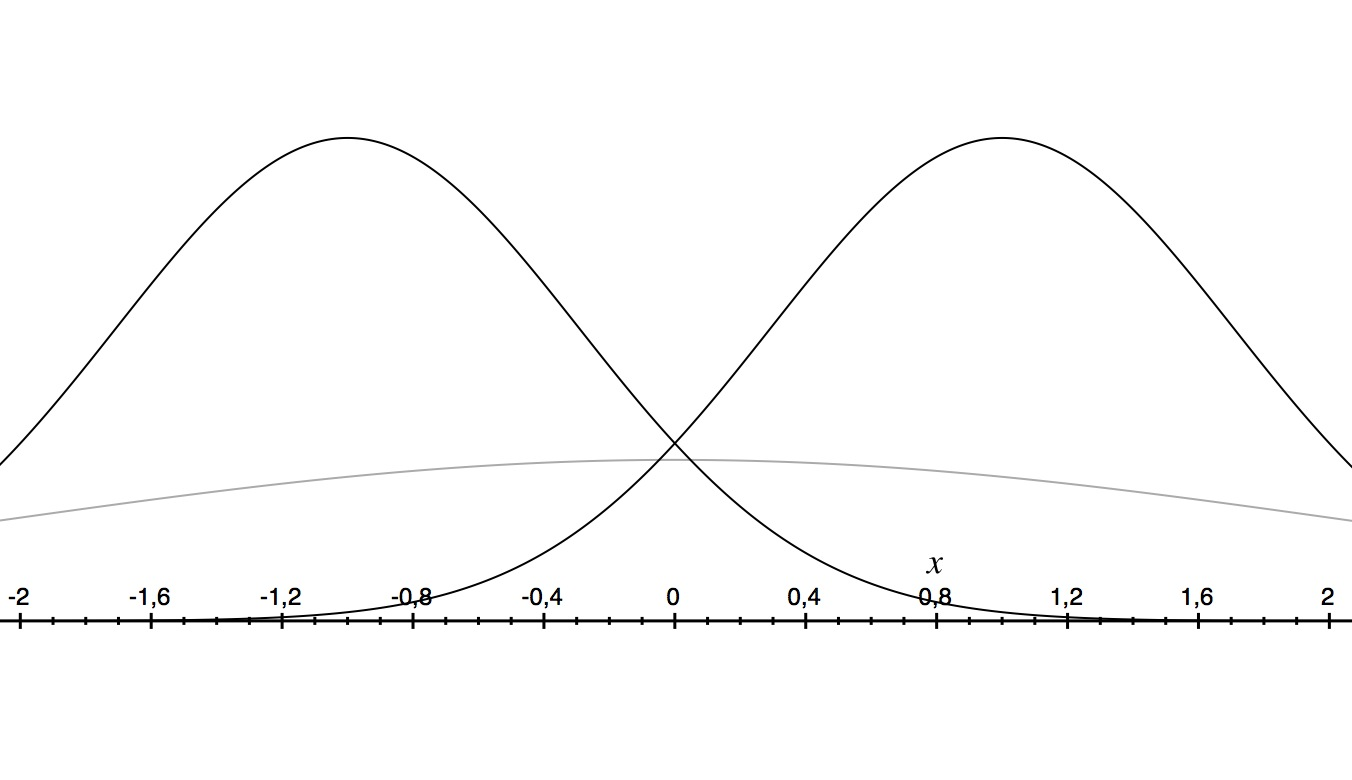
\includegraphics[width=50mm]{figures/diversity2.jpg}
                \caption{{\bf High} diversity}
        \end{subfigure}
       ~ %add desired spacing between images, e. g. ~, \quad, \qquad, \hfill etc.
          %(or a blank line to force the subfigure onto a new line)
        \begin{subfigure}[b]{0.45\textwidth}
		 \centering
                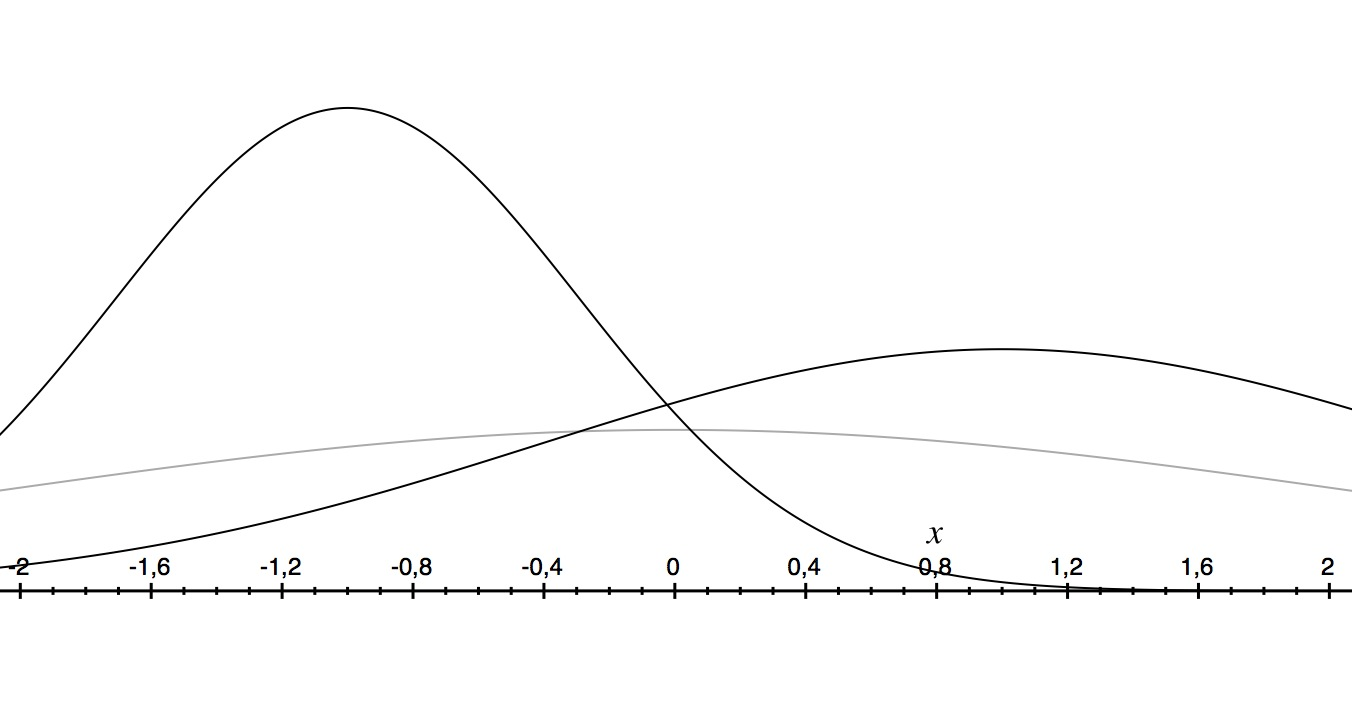
\includegraphics[width=50mm]{figures/diversity3.jpg}
\caption{Low diversity}
        \end{subfigure}
       ~ %add desired spacing between images, e. g. ~, \quad, \qquad, \hfill etc.
          %(or a blank line to force the subfigure onto a new line)
        \begin{subfigure}[b]{0.45\textwidth}
		 \centering
                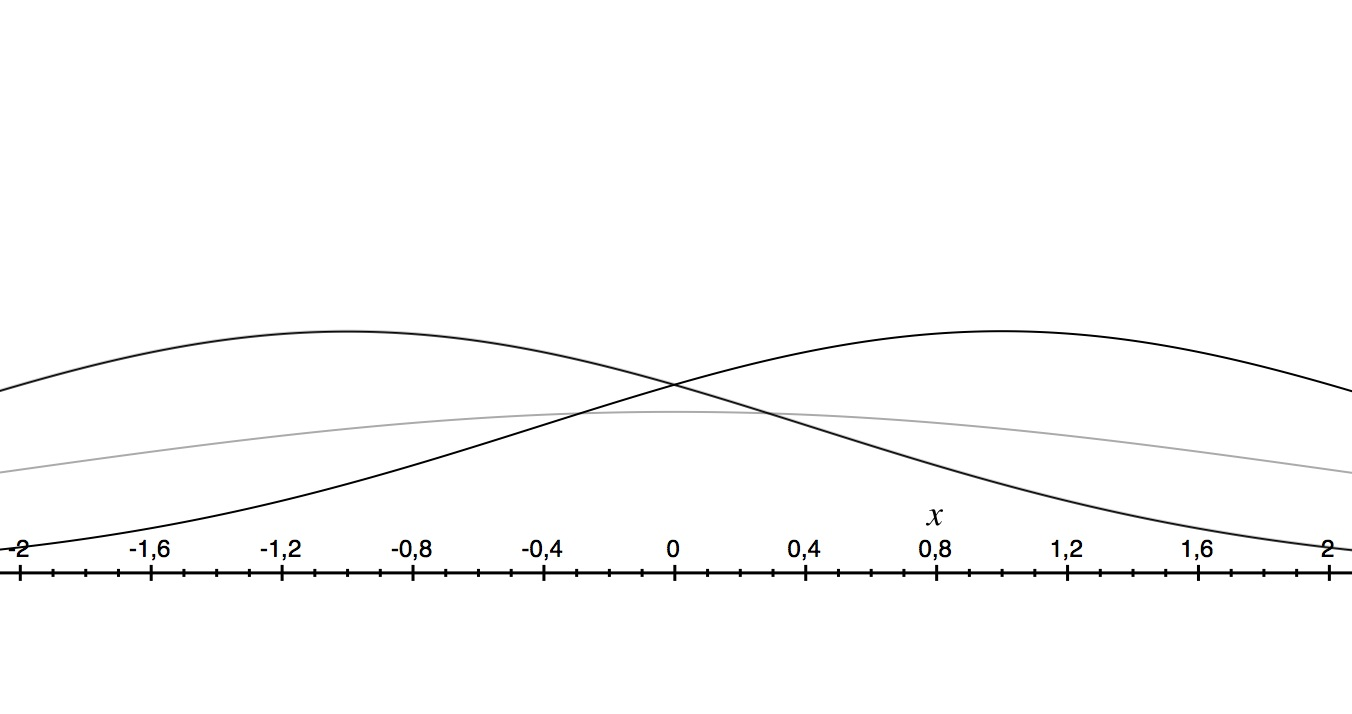
\includegraphics[width=50mm]{figures/diversity4.jpg}
\caption{Low diversity}
        \end{subfigure}
\end{figure}
\end{frame}

\subsection{Population Diversity (digression)}

\begin{frame}
\frametitle{Population Diversity (digression)}
\begin{itemize}
\item Information Diversity works well with the bag of words
  interpretation. 
\item However, its relation with entropy suggests a
  connection with population diversity.
\item What is the role of the prior distribution in a population?
\item Why is the prior uniform in the theorem? What if it is not?
\end{itemize}
\end{frame}

\begin{frame}
\frametitle{Generative Population Model}
\begin{itemize}
\item Consider a population $S$ of
  organisms assigned species from the set $T$. $S$ was generated from a universe
  $U$ by:
\begin{enumerate}
\item We draw an element $u$ uniformly from $U$. Let $t\in
T$ be the species assignment for $u$.
\item We choose to add $u$ to
$S$ with probability $p_{S,t}$ (depending only on the species
assignment of $u$).
\end{enumerate}
\item We will assume that:
\begin{enumerate}
\item $S$ is large enough that its species
  distribution has {\em converged}.
\item $U$ is large enough compared to $S$, so that sampling from it
  does not noticeably affect its species distribution.
\end{enumerate}
\end{itemize}
\end{frame}

\begin{frame}
\frametitle{Axiomatic Definition of Diversity}
We will now postulate
the following general properties that a diversity measure
should have in this model:
\begin{enumerate}
\item Given a fixed set of parameters $p_{S,t}$ for the generative
  process, the population diversity does not depend on the species
  distribution of the universe.
\item If the species distribution of the universe is uniform, then we can
  revert to a standard model of population diversity. In our case, we
  will use Shannon entropy.
\end{enumerate}
Here, the universe distribution corresponds to a prior distribution.
\end{frame}

\begin{frame}
\frametitle{Population Diversity with Prior Distribution}
\bet
A population that is uniformly sampled from the universe has
  highest diversity. 
\eet
\bet
Let $S$ be a population sampled within universe $U$, where $P_S$ and
$P_U$ are the species distributions of $S$ and $U$,
respectively. Denote $T$ as the set of species. Let $Q$ be a species
distribution such that
\[Q(t)=\frac{P_S(t)(P_U(t))^{-1}}{\sum_{v\in T} P_S(v)(P_U(v))^{-1}}.\]
Then, the diversity of $S$ within $U$ is equal to $H(Q)$.
\eet
\end{frame}

\begin{frame}
\frametitle{Jensen-Shannon Population Diversity}
\bed
We define the Jensen-Shannon Population Diversity of
$\cP=\{P_1,...,P_k\}$ with respect to prior $P$ as
$\mbox{JSPD}_P(\cP)=D_{JS}(\Sigma d_i P_i)$ 
where $d_{i}=\frac{2^{D_{i}}}{\sum 2^{D_{j}}}$ are the normalized
{\bf exponentiated importances}.
\eed
\bet
Let $\cP$ be such that each $P_i$ has a singleton support. Then, given
$P$ as the 
prior,  $JSPD_P(\cP)$ is equal to the diversity of $\cP$ as a
population within a universe with species distribution $P$.
\eet
\end{frame}

\subsection{Text Diversity}

\begin{frame}
\frametitle{Choosing Word Representations}
\begin{itemize}
\item We decided to use Jensen-Shannon Information Diversity, given
  word representations $\cP=\{P_1,...,P_k\}$, and a prior $P$.
\item Given $W=\{w_1,...,w_k\}$, how should the Observer choose $P_{i}$, knowing
  $\cM_{|V|\times|T|}$?

{\bf Intuition:} We can use the row of $\cM_{|V|\times|T|}$ that
corresponds to $w_i$, normalized to a distribution.
\item What should the prior $P$ be?

{\bf Intuition: (WRONG)} We can use the average of all word representation vectors.
\end{itemize}
\end{frame}

\begin{frame}
\frametitle{Capturing Topic Similarity}
\begin{itemize}
\item {\bf Problem:} A distributional representation of a word does
  not capture the relations between topics.
\item Suppose we are given a topic similarity matrix
  $\cS_{|T|\times|T|}$, where $\cS_{ij}$ is the number indicating
  the degree of similarity between topics $i$ and $j$. 
\item Let $\tilde{\cS}$ be the matrix $\cS$ with all the rows normalized as
  distributions. 
\item Given $P_i$, we can now consider $\tilde{P_i}=P_i\tilde{S}^T$, which
  essentially diffuses $P_i$ accross similar topics.
\end{itemize}
\end{frame}

\begin{frame}
\frametitle{Capturing Topic Similarity, cont.}
\begin{itemize}
\item We can think of $\tilde{P_i}$ as Observer's {\em second order}
  topic correlation distribution for a given word.
\item To obtain the appropriate prior as average of the word
  representations, we can simply diffuse the old prior
  $\tilde{P}=P\tilde{S}^T$. 
\item To choose a good matrix $\cS$, we can use the topic model. For
  example, we can apply cosine similarity between topic document
  vectors based on the LDA. 
\item More appropriate choices of $\cS$ still need to be examined.
\end{itemize}
\end{frame}

\begin{frame}
\frametitle{Sample Size Bias}
\begin{itemize}
\item {\bf Problem:} Some of the row vectors in $\cM$ may not have
  enough data points to properly estimate the topic distribution.
\item We can treat the Observer as a Bayesian that has a Dirichlet
  prior (concentrated around the prior topic distribution
  $\tilde{P}$). 
\item This leads to a simple smoothing operation:
\begin{equation}
\widehat{P}_i=\frac{\alpha \tilde{P}+ \mu_i \tilde{P}_i}{\alpha+\mu_i}.
\end{equation}
\item Here, $\mu_i$ is the frequency of word $w_i$ in the LDA corpus,
  and $\alpha$ is the prior strength.
\end{itemize}
\end{frame}

\begin{frame}
\frametitle{Conditioning on the Context}
\begin{itemize}
 \item {\bf Problem:} The word $w_i$ has a specific meaning inside of
   $W=\{w_1,...,w_k\}$, that can be significantly different than its
   meaning out of context. 
\item Denote $W_{\bar{i}}=W-\{w_i\}$. By $\widehat{P}_{W_{\bar{i}}}$, we denote
  the mixture distribution $\Sigma d_j\widehat{P}_j$ for $W_{\bar{i}}$
  (as defined for JSID).
\item Suppose that matrix $\cM$ was generated from the same topics, however
  distributed not as $\tilde{P}$ but as
  $\widehat{P}_{W_{\bar{i}}}$.
\item What would be the new topic distribution for $w_i$?
\end{itemize}
\end{frame}

\begin{frame}
\frametitle{Conditioning on the Context, cont.}
\bet
Let $\tilde{P},\widehat{P}_{i}, \widehat{P}_{W_{\bar{i}}}$ be the
topic prior, the general
topic distribution for $w_i$, and the context distribution,
respectively. Then, the context-dependent distribution of $w_i$ will
be 
\vspace{-2mm}
\begin{equation*}
P^{W_{\bar{i}}}_{i}(t)\propto \frac{\widehat{P}_{W_{\bar{i}}}(t)}{\tilde{P}(t)}\widehat{P}_{i}(t).
\end{equation*}
\eet
\bed
We use smoothing again, to obtain the Observer's distribution:
\vspace{-2mm}
\[\widehat{P}^{W_{\bar{i}}}_{i}(t)\propto \beta \widehat{P}_{i}\!(t)
+\frac{\widehat{P}_{W_{\bar{i}}}(t)}{\tilde{P}(t)}\widehat{P}_{i}(t).\] 
\eed
\end{frame}

\section{Experiments}

\begin{frame}
\frametitle{Data Sets}
\begin{enumerate}
\item Interesting iPhone cases on eBay.
  \begin{itemize}
  \item We hired workers from {\em AMT} to label a collection
of iPhone cases found on {\em Pinterest} and {\em
  eBay's}.
\item The final data-set consists of 2179 positive and 9770 negative instances for
a total of 11,949 instances, with product title used as input. 
\item The topic model was trained using Mallet on 2 million product
  titles, grouped by categories into 800 documents.
\end{itemize}
\item NSF proposal abstracts (61,902 total, 200-300 words each).
\begin{itemize}
\item We used this set 
for training a topic model.
\item To get labeled data, we had to generate $5000$ artificial
  labeled examples, by mixing random abstracts. 
\end{itemize}
\end{enumerate}
\end{frame}

\subsection{Unsupervised Evaluation}

\begin{frame}
\frametitle{Unsupervised Evaluation}
\begin{itemize}
\item We draw an ROC curve by thresholding diversity
  over labeled examples. 
\item As baselines, we use probabilistic diversity
  measures with input being a topic distribution for  given example,
  inferred from the LDA model using Mallet.
\item Baseline measures:
\begin{enumerate}
\item Shannon Entropy - commonly used measure of diversity.
\item Shannon Entropy with topic distributions diffused using the topic
  similarity matrix. 
\item Rao Diversity, as described in [?] (which also uses the same
  topic similarity matrix). 
\end{enumerate}
\end{itemize}
\end{frame}

\begin{frame}
\frametitle{Unsupervised Results: eBay}
\begin{figure}
        \centering
        \begin{subfigure}[b]{0.45\textwidth}
                \centering
                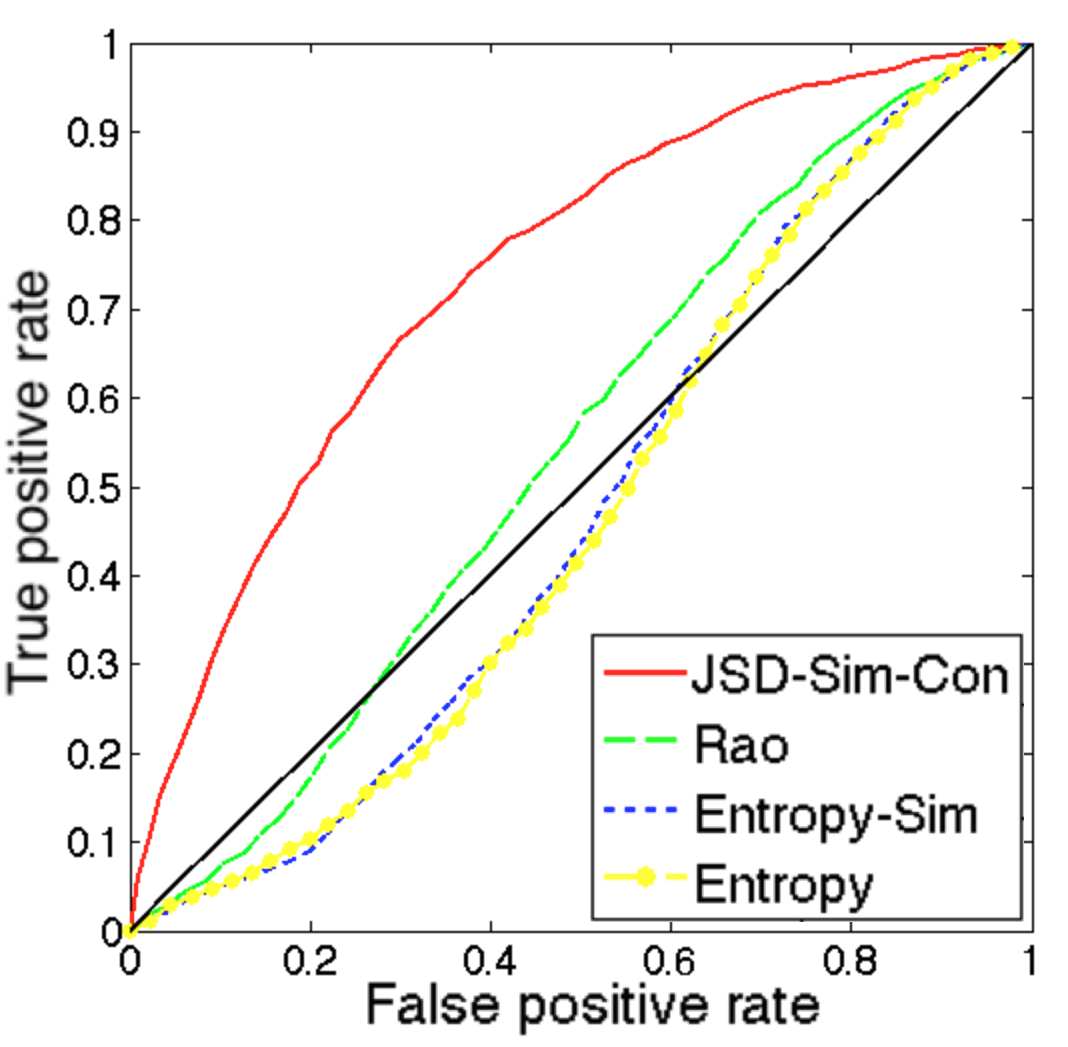
\includegraphics[width=40mm]{figures/phonecases-comparison-kopia.png}
               \caption{eBay (baseline)}
                \label{fig:phonecases-comparison}
        \end{subfigure}%\qquad
              ~ %add desired spacing between images, e. g. ~, \quad, \qquad, \hfill etc.
          %(or a blank line to force the subfigure onto a new line)
        \begin{subfigure}[b]{0.45\textwidth}
                \centering
                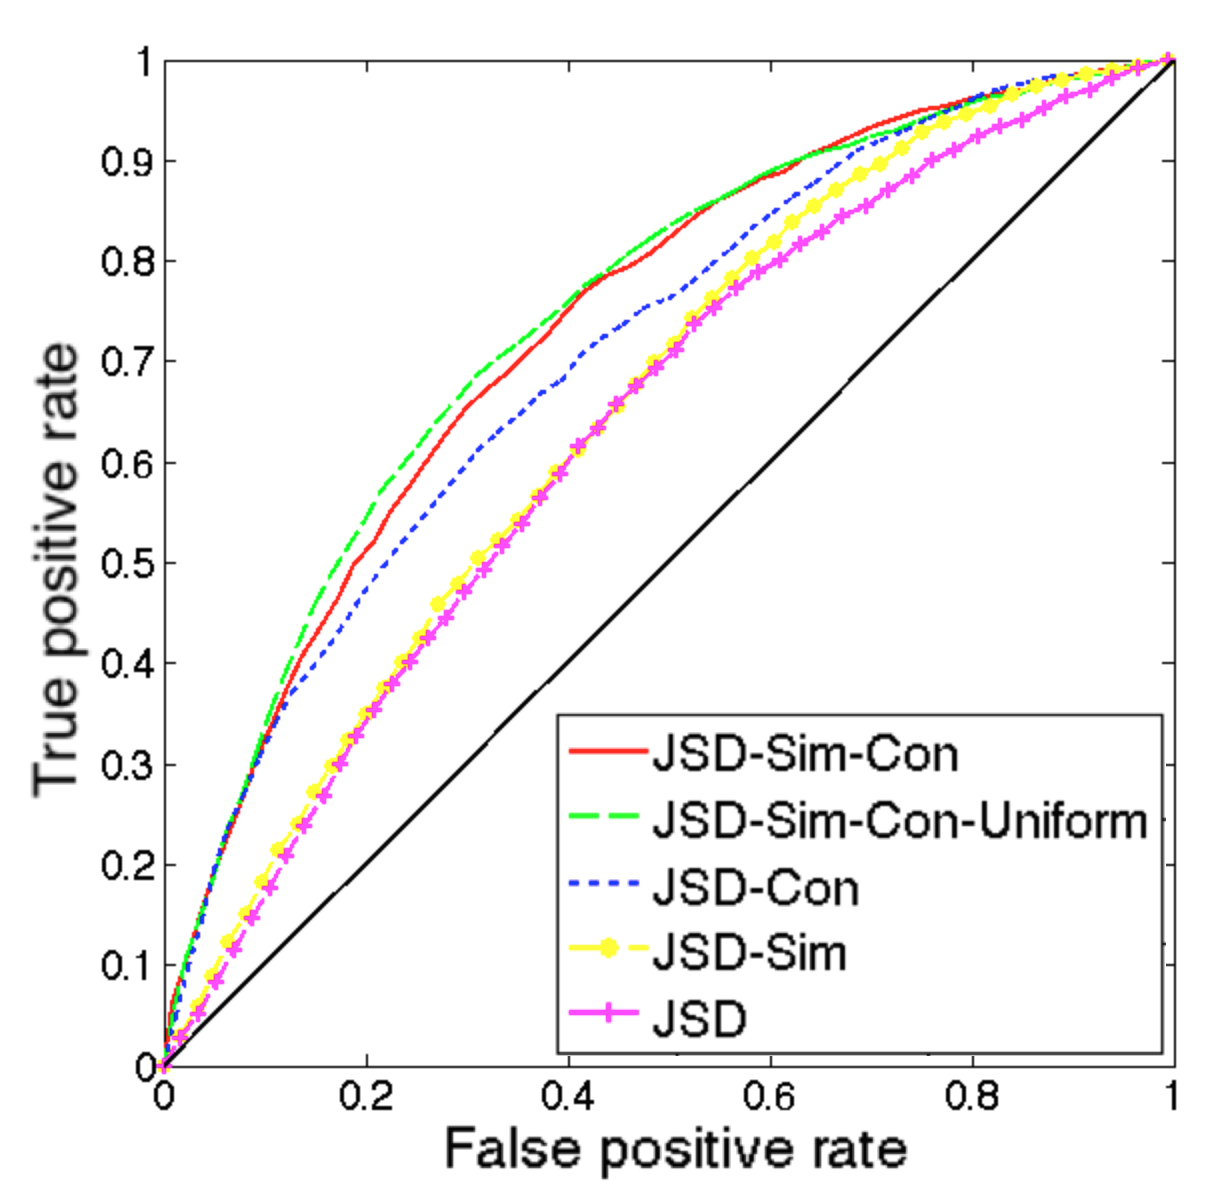
\includegraphics[width=40mm]{figures/phonecases-breakdown-kopia.png}
                \caption{eBay (JSD)}
                \label{fig:phonecases-breakdown}
        \end{subfigure}\nobreak
\end{figure}
\end{frame}

\begin{frame}
\frametitle{Unsupervised Results: NSF Abstracts}
\begin{figure}
        \begin{subfigure}[b]{0.45\textwidth}
                \centering
                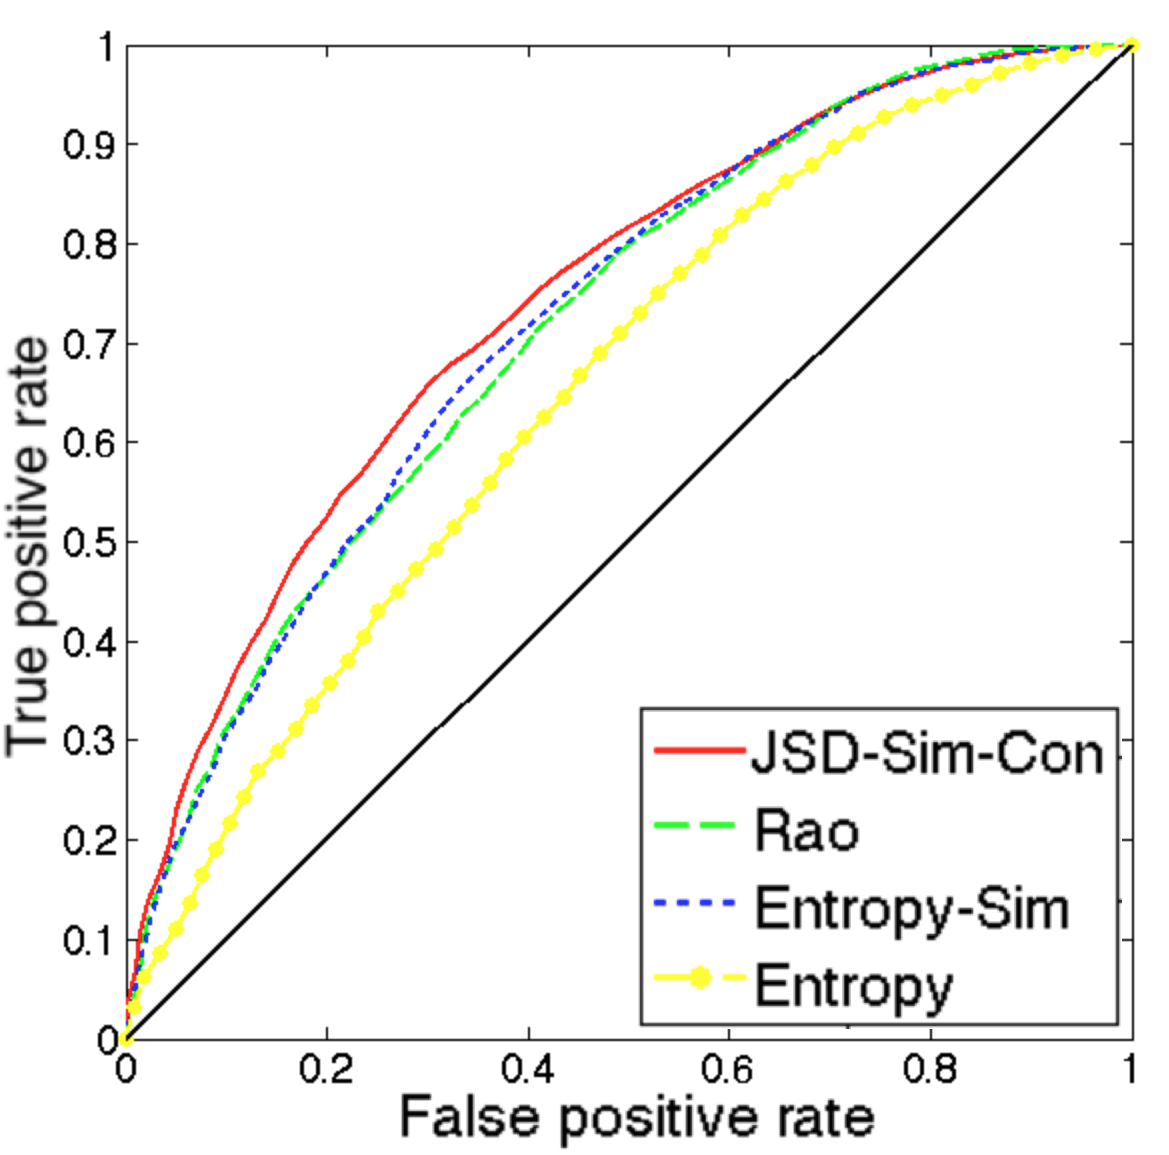
\includegraphics[width=40mm]{figures/nsf-comparison-kopia.png}
                \caption{NSF (baseline)}
                \label{fig:nsf-comparison}
        \end{subfigure}%\qquad
        ~ %add desired spacing between images, e. g. ~, \quad, \qquad, \hfill etc.
          %(or a blank line to force the subfigure onto a new line)
        \begin{subfigure}[b]{0.45\textwidth}
        	        \centering
                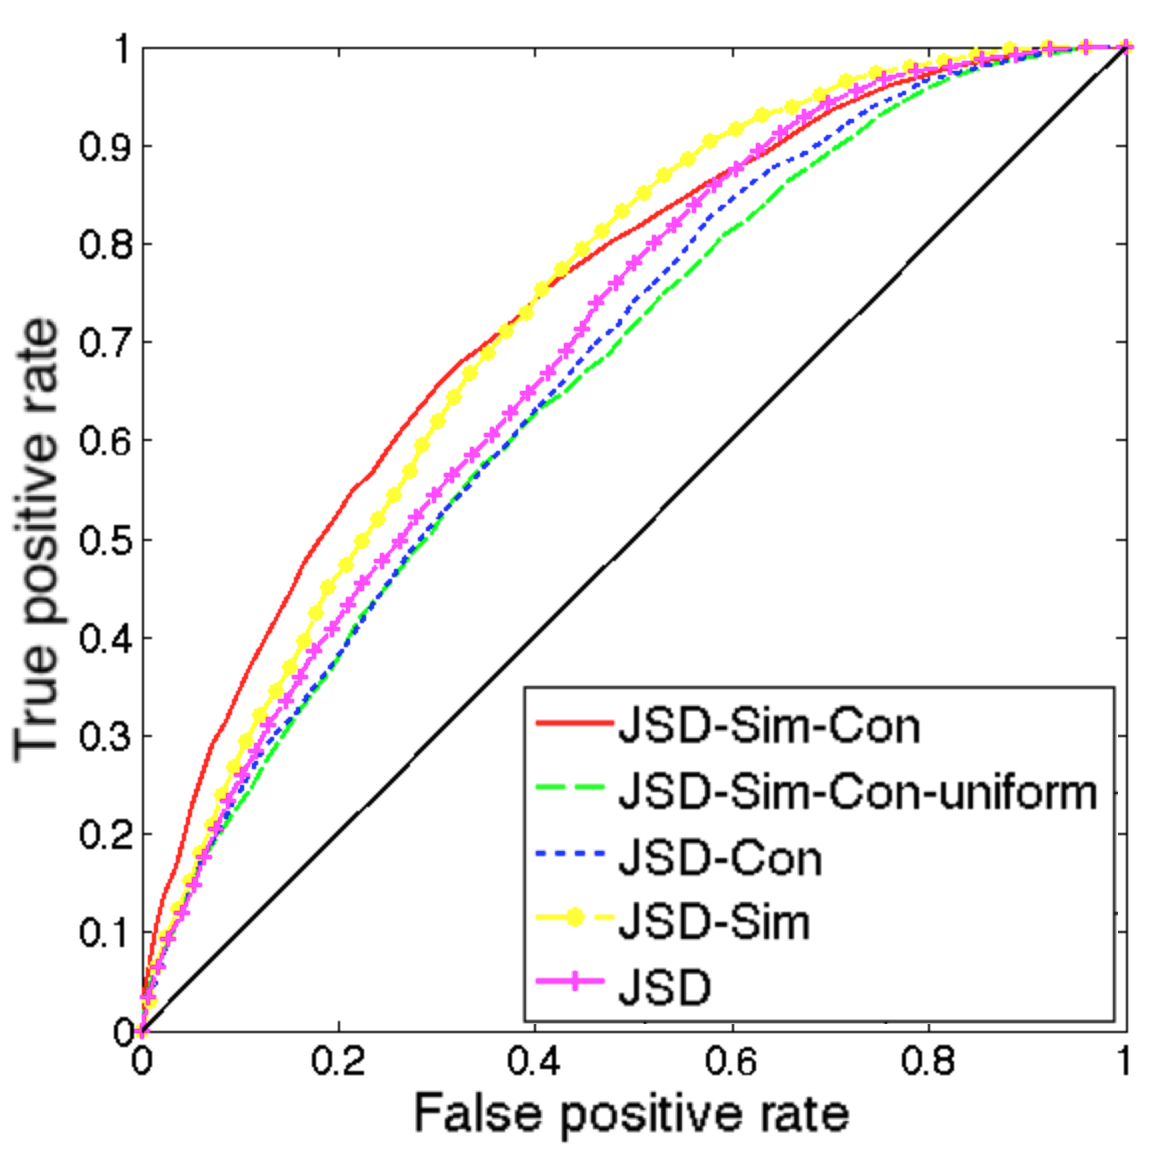
\includegraphics[width=40mm]{figures/nsf-breakdown-kopia.png}
               \caption{NSF (JSD)}
                \label{fig:nsf-breakdown}
        \end{subfigure}
\end{figure}
\end{frame}

\subsection{Supervised Evaluation}

\begin{frame}
\frametitle{Supervised Evaluation}
\begin{itemize}
\item We use an unnormalized form of the mixture topic distribution,
  $\tilde{M}=\Sigma D_i\hat{P}_i^{W_{\bar{i}}}$, as a feature vector
  for an SVM classifier trained on eBay data.
\item The results are averaged over five cross-validation $60\%$
  splits.
\item Baselines:
\begin{enumerate}
\item {\em Recursive Auto-Encoders} with Word2Vec - a deep learning approach
  using the framework from [?] (300 dimensions).
\item {\em Latent Semantic Indexing} - forming a document-term matrix
  and performing SVD. (200 dimensions).
\end{enumerate}
\end{itemize}
\end{frame}

\begin{frame}
\frametitle{Supervised Results}
\begin{table}[t]
%\caption{Classification results for the eBay dataset.}
\label{tab:classification-results}
\vspace{-4mm}
\begin{center}
\begin{tabular}{|l|c|c|c|c|}
\hline
&Precision & Recall & F1 & Accuracy
\\ \hline 
JSID         &$\mathbf{0.714}$&$0.597$&$0.650$& $\mathbf{0.8828}$\\
RAE             &$0.676$&$\mathbf{0.666}$&$\mathbf{0.671}$&$0.8809$ \\
LSI             &$0.676$&$0.633$&$0.654$&$0.8778$\\
\hline
\end{tabular}
\end{center}
\end{table}
\begin{itemize}
\item Our method outperforms the baselines on both accuracy and
  precision.
\item Note, that in this type of problem precision is much more
  important than recall, since we are interested only in a small
  selection of good diverse examples.
\item We obtain a good feature selection technique as a by-product
  of our diversity measure.
\end{itemize}
\end{frame}

\subsection{Conclusions}

\begin{frame}
\frametitle{Conclusions}
\begin{itemize}
\item We proposed a new diversity measure, that generalizes entropy.
\item We showed, how it can be applied to text data, using specific
  enhancements to the general definition.
\item The results show that the measure performs well for text of
  various sizes, which is especially significant when the text is very
  short.
\item As a by-product of the approach we get feature vectors that
  performed well in a classification task.
\end{itemize}
\end{frame}

\begin{frame}
\frametitle{Future Work}
\begin{itemize}
\item Explore interestingness retrieval in other collections of short pieces of
  text (e.g. Twitter messages).
\item Try JSID feature vectors on other classification tasks.
\item Gain a deeper theoretical understanding of JSID and JSPD.
\item Find other applications for measuring diversity of a set of
  distributions.
\end{itemize}
\end{frame}

\begin{frame}

\centering{\bf \LARGE Thank you}

\end{frame}

\end{document}